\documentclass{../myclass}
\usepackage[polish]{babel}

\begin{document}
\begin{center}
    \Large \textbf{Laboratorium 5.}\\
    \large
    \textsc{Algebra H-macierzy}\\
    \normalsize
    Bartosz Hanc
\end{center}    

\section{Wstęp}

Celem ćwiczenia było napisanie algorytmów mnożenia macierzy skompresowanej przez wektor oraz
mnożenia dwóch macierzy skompresowanych. Dodatkowo należało dla macierzy rzadkich o strukturze
opisującej topologię siatki trójwymiarowej zbudowanej z sześciennych komórek zmierzyć czasy mnożenia
przez losowy wektor i przez samą siebie dla siatek o rozmiarach \(4\times 4\times 4\), \(8 \times 8
\times 8\) oraz \(16\times16\times16\) (macierzy rozmiaru \(64 \times64\), \(512\times 512\), \(4096
\times 4096\)).

\section{Kod rozwiązania}

Funkcja \pythoninline{mvmult(v: Node, X: np.ndarray, rev: bool)} implementuje mnożenie macierzy
skompresowanej przez wektor. Argument typu \pythoninline{rev: bool} określa czy wykonujemy mnożenie
z prawej \(H_vX\) (\pythoninline{rev=False}), czy z lewej strony \(XH_v\) (\pythoninline{rev=True}).

\begin{python}
def mvmult(v: Node, X: np.ndarray, rev=False) -> np.ndarray:
    if not v.next:
        if v.rank == 0:
            return np.zeros(X.shape)
        if rev:
            return X @ v.U @ np.diag(v.D) @ v.V
        return v.U @ np.diag(v.D) @ v.V @ X

    k = X.shape[1] if rev else X.shape[0]
    X1 = X[:, : k // 2] if rev else X[: k // 2, :]
    X2 = X[:, k // 2 :] if rev else X[k // 2 :, :]

    Y11 = mvmult(v.next[0], X1, rev)
    Y12 = mvmult(v.next[2 if rev else 1], X2, rev)
    Y21 = mvmult(v.next[1 if rev else 2], X1, rev)
    Y22 = mvmult(v.next[3], X2, rev)

    return np.hstack((Y11 + Y12, Y21 + Y22)) \ 
           if rev else np.vstack((Y11 + Y12, Y21 + Y22))
\end{python}
Funkcja \pythoninline{mmmult(v: Node, w: Node)} implementuje z kolei mnożenie dwóch macierzy
skompresowanych reprezentowanych przez korzenie \pythoninline{v: Node}, \pythoninline{w: Node}
macierzy hierarchicznych.

\newpage
\begin{python}
def mmmult(v: Node, w: Node) -> np.ndarray:
    zstack = lambda a, b, c, d: \
        np.vstack((np.hstack((a, b)), 
                   np.hstack((c, d))))

    if v.rank == 0 or w.rank == 0:
        return np.zeros((v.side, w.side))

    if not v.next and not w.next:
        return v.U @ np.diag(v.D) @ v.V @ w.U @ np.diag(w.D) @ w.V

    if v.next and w.next:
        a1, a2, a3, a4 = v.next
        b1, b2, b3, b4 = w.next
        return zstack(
            mmmult(a1, b1) + mmmult(a2, b3),
            mmmult(a1, b2) + mmmult(a2, b4),
            mmmult(a3, b1) + mmmult(a4, b3),
            mmmult(a3, b2) + mmmult(a4, b4))

    if not v.next and w.next:
        k = v.side
        b1, b2, b3, b4 = w.next
        U, V = v.U @ np.diag(v.D), v.V
        A1 = U[: k // 2, :] @ V[:, : k // 2]
        A2 = U[: k // 2, :] @ V[:, k // 2 :]
        A3 = U[k // 2 :, :] @ V[:, : k // 2]
        A4 = U[k // 2 :, :] @ V[:, k // 2 :]
        return zstack(
            mvmult(b1, A1, rev=True) + mvmult(b3, A2, rev=True),
            mvmult(b2, A1, rev=True) + mvmult(b4, A2, rev=True),
            mvmult(b1, A3, rev=True) + mvmult(b3, A4, rev=True),
            mvmult(b2, A3, rev=True) + mvmult(b4, A4, rev=True))

    if v.next and not w.next:
        k = w.side
        a1, a2, a3, a4 = v.next
        U, V = w.U @ np.diag(w.D), w.V
        B1 = U[: k // 2, :] @ V[:, : k // 2]
        B2 = U[: k // 2, :] @ V[:, k // 2 :]
        B3 = U[k // 2 :, :] @ V[:, : k // 2]
        B4 = U[k // 2 :, :] @ V[:, k // 2 :]
        return zstack(
            mvmult(a1, B1) + mvmult(a2, B3),
            mvmult(a1, B2) + mvmult(a2, B4),
            mvmult(a3, B1) + mvmult(a4, B3),
            mvmult(a3, B2) + mvmult(a4, B4))
\end{python}
\newpage
\section{Wyniki}

Zgodnie z poleceniem wygenerowano macierze o strukturze opisującej topologię trójwymiarowej siatki
zbudowanej z komórek sześciennych o rozmiarach \(2^{3k} \times 2^{3k}\) dla \(k\in\{2,3,4\}\).
Następnie dokonano ich kompresji do macierzy hierarchicznych korzystając z funkcji
zaimplementowanych w ramach laboratorium 3. Poniżej na Rysunkach \ref{fig:1}, \ref{fig:2},
\ref{fig:3} przedstawiono wizualizacje uzyskanych macierzy hierarchicznych.

\begin{figure}[ht]
    \centering
    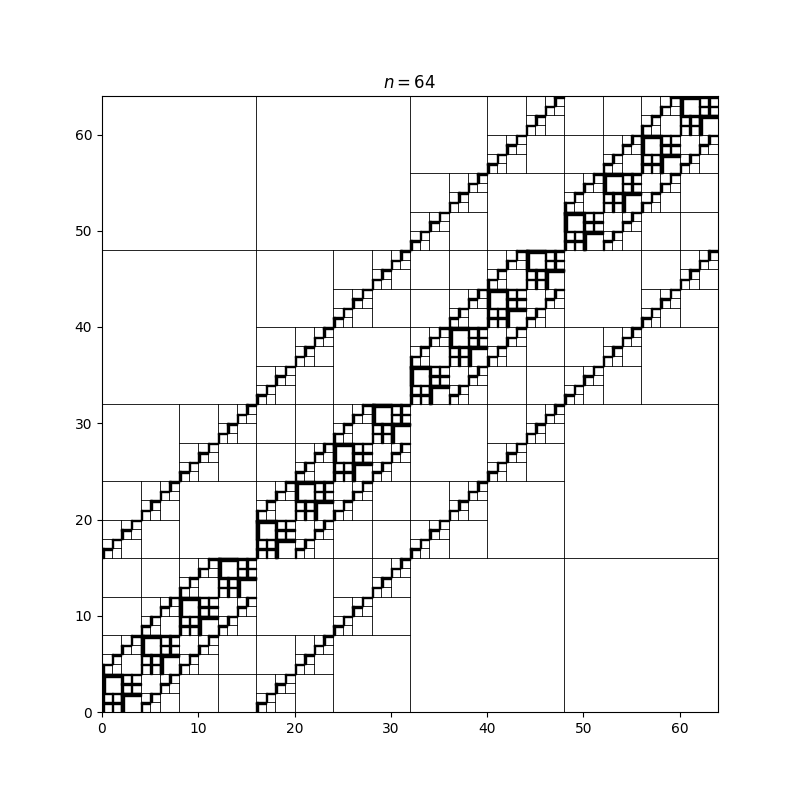
\includegraphics[width=0.55\textwidth]{0_bp_hm.png}
    \caption{Macierz opisująca siatkę \(4\times4\times4\) po kompresji}
    \label{fig:1}
\end{figure}

Dla wygenerowanych macierzy sprawdzono następnie poprawność zaimplementowanych funkcji porównując otrzymany wynik z wynikiem bezpośredniego mnożenia macierzy.
\begin{python}
for A in As:
    v = CreateTree(A, r=1, eps=1e-3)
    X = np.random.random((A.shape[0], 1))
    print(np.allclose(A @ X, mvmult(v, X, rev=False)))
    print(np.allclose(X.T @ A, mvmult(v, X.T, rev=True)))

for A in As:
    v = CreateTree(A, r=1, eps=1e-3)
    print(np.allclose(A @ A, mmmult(v, v)))

>>> True (x9)
\end{python}

\begin{figure}[h!]
    \centering
    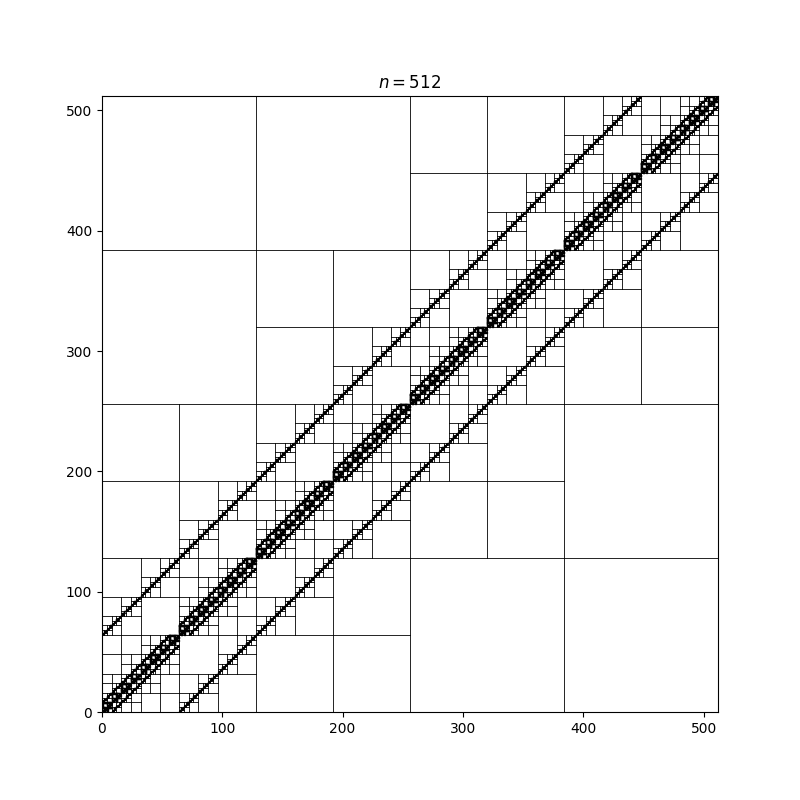
\includegraphics[width=0.55\textwidth]{1_bp_hm.png}
    \caption{Macierz opisująca siatkę \(8\times8\times8\) po kompresji}
    \label{fig:2}
\end{figure}

\begin{figure}[h!]
    \centering
    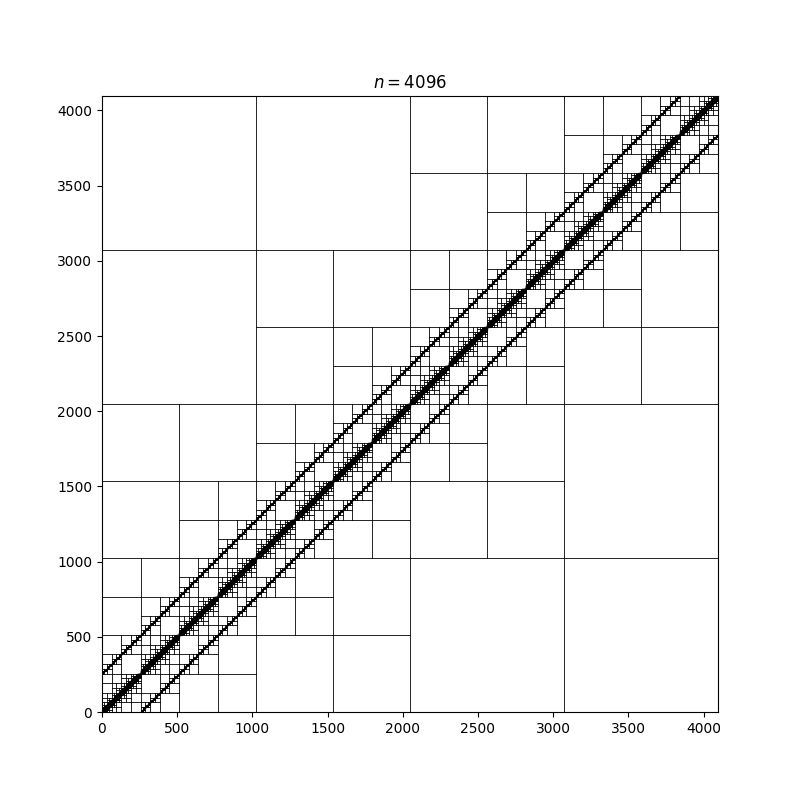
\includegraphics[width=0.55\textwidth]{2_bp_hm.png}
    \caption{Macierz opisująca siatkę \(16\times16\times16\) po kompresji}
    \label{fig:3}
\end{figure}
\newpage
Następnie zmierzono czasy mnożenia macierzy przez losowy wektor oraz przez siebie. Uzyskane wyniki
przedstawiono na Rysunkach \ref{fig:4} i \ref{fig:5}. Do uzyskanych punktów pomiarowych dopasowano
krzywe postaci \(t(n) = \alpha n^\beta\).

\begin{figure}[ht]
    \centering
    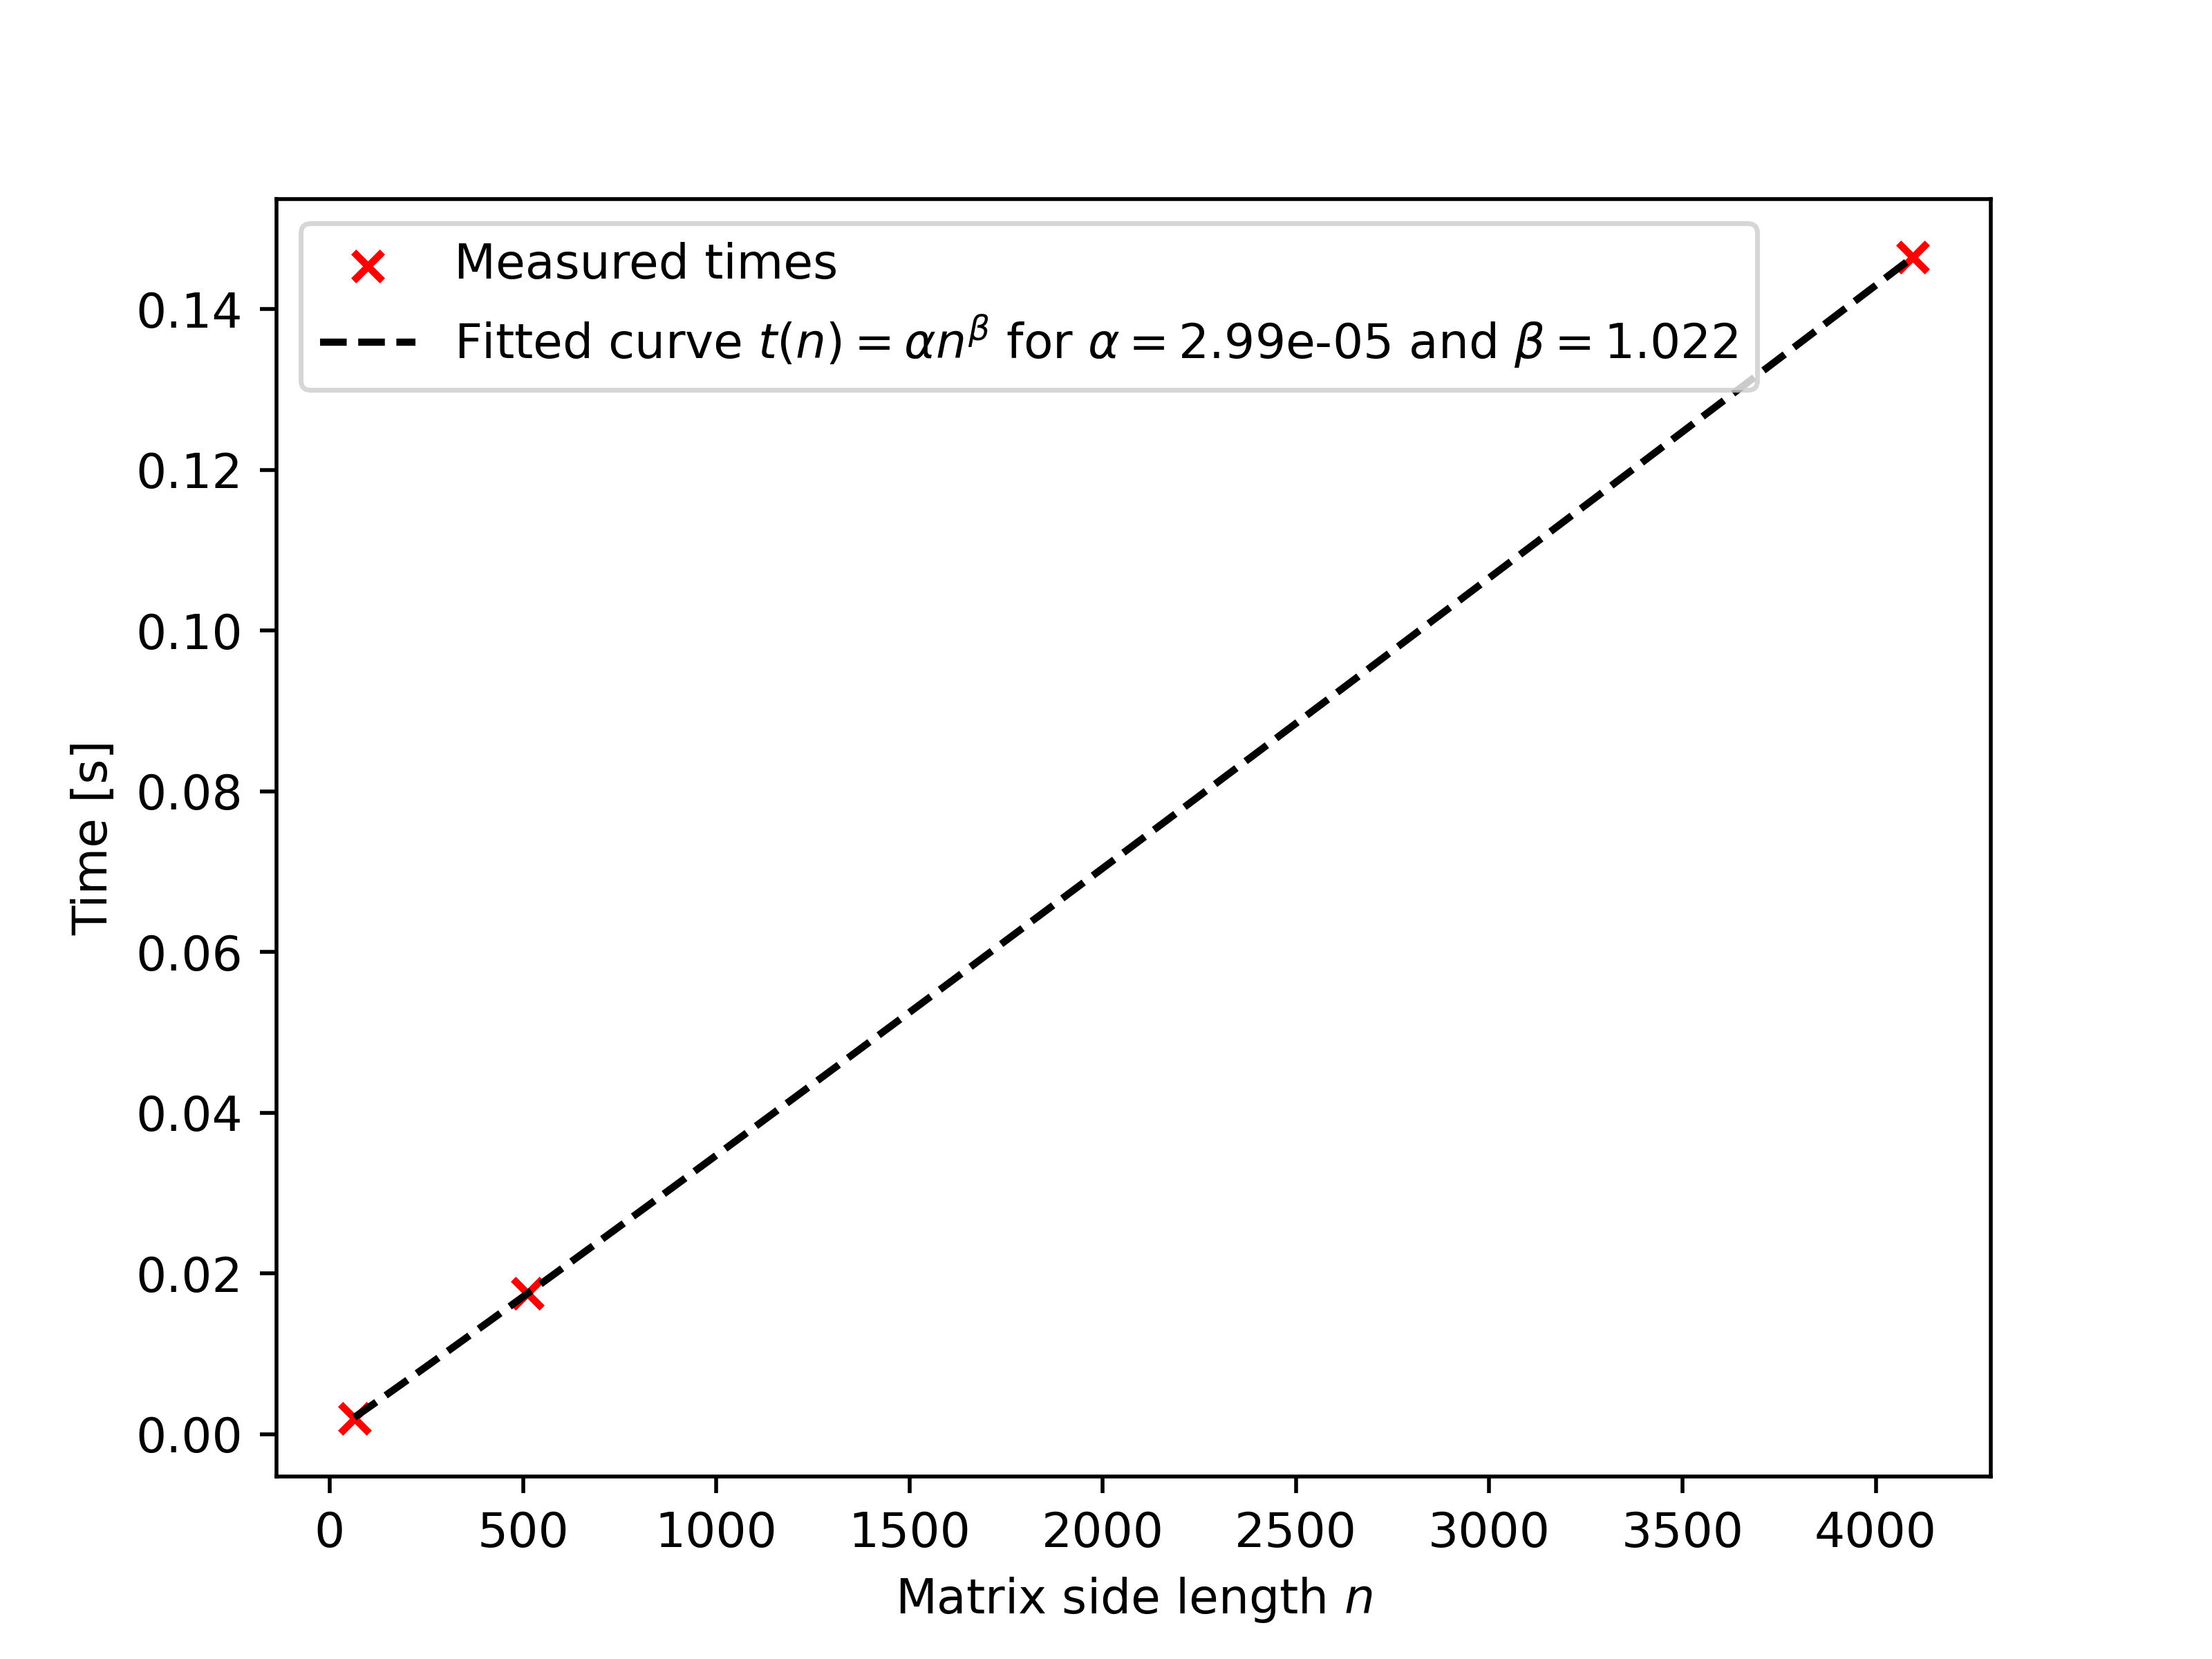
\includegraphics[width=0.8\textwidth]{mvtimes.png}
    \caption{Czasy mnożenia macierzy hierarchicznej przez wektor}
    \label{fig:4}
\end{figure}

\begin{figure}[ht]
    \centering
    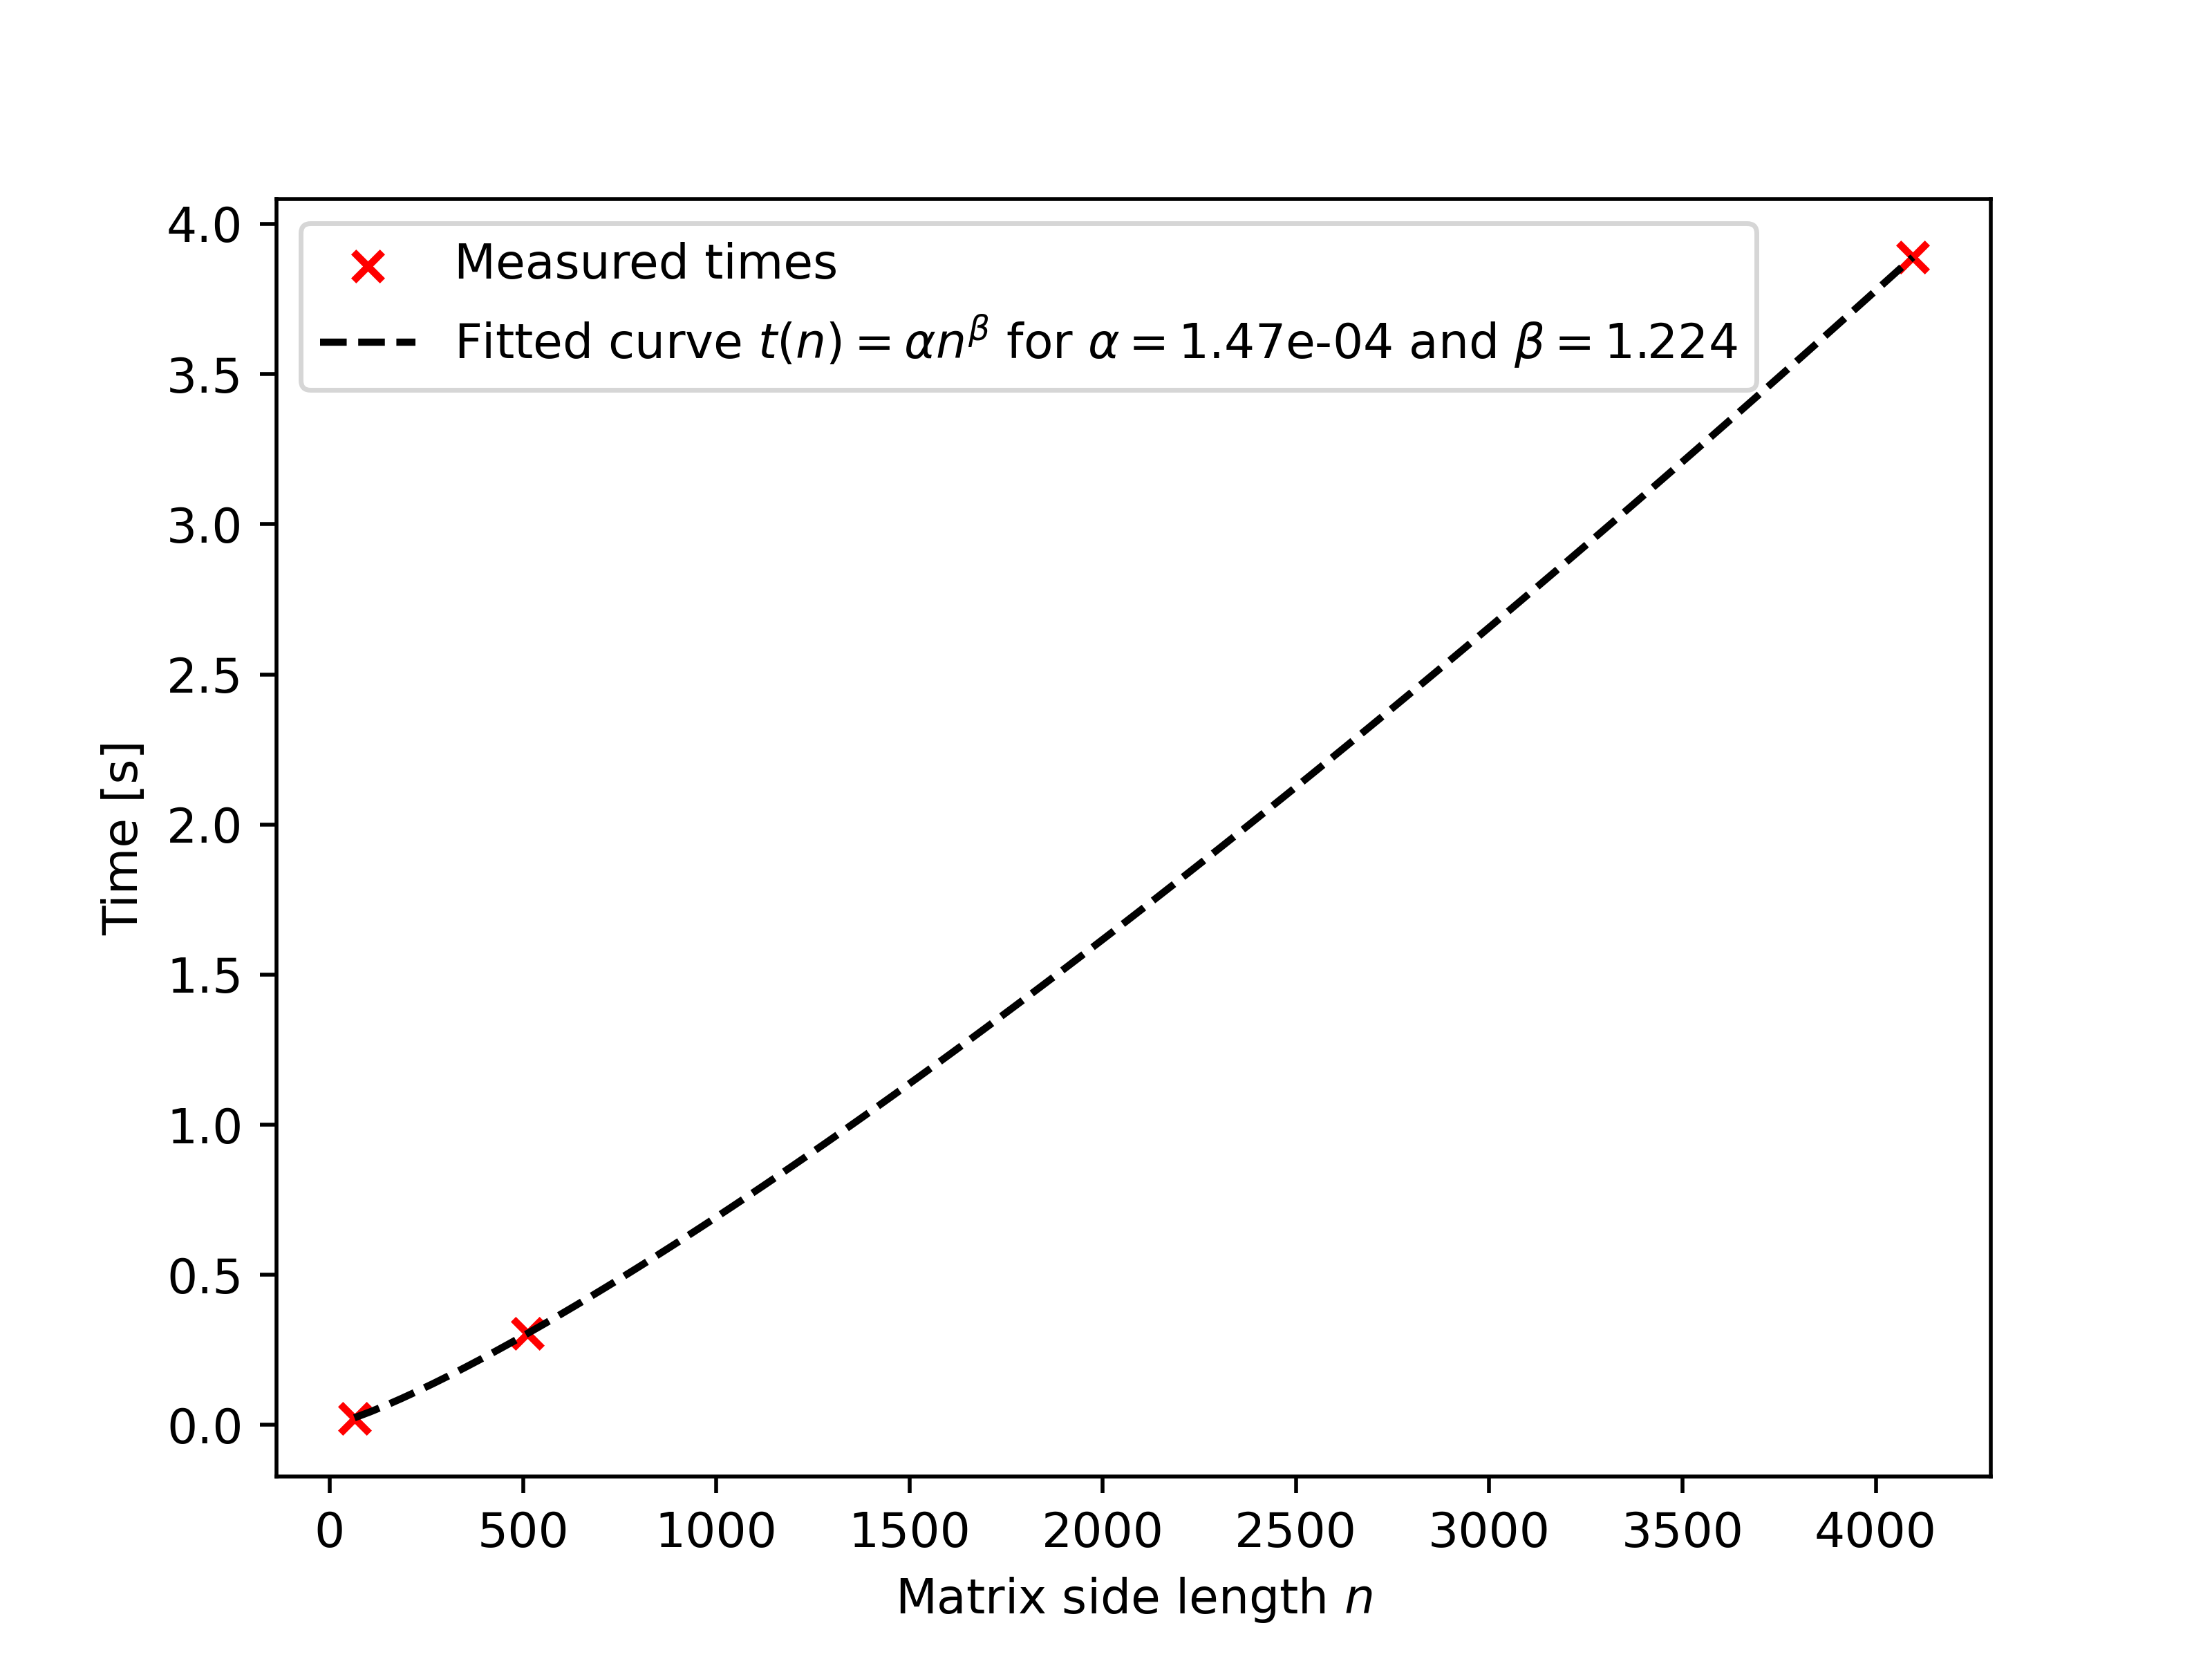
\includegraphics[width=0.8\textwidth]{mmtimes.png}
    \caption{Czasy mnożenia macierzy hierarchicznej przez samą siebie}
    \label{fig:5}
\end{figure}


\end{document}